%MultiSeq Manual 8/1/2005
%Root document / outline of the entire manual
 
\documentclass[letterpaper]{article}
\usepackage{graphicx, wrapfig, floatflt, html}
\begin{document}


\pagestyle{headings}

%\input{macros}
%\input{title}


\setcounter{tocdepth}{3}
% \tableofcontents
% \pagebreak

%Introduction which gives an in-depth description of what MultiSeq does 
%Perhaps we could take this out of Elijah's paper
% Necessary components to run MultiSeq - VMD 1.8.3a? installation / BLAST on the hard drive
\label{unit0}
%Introduction which gives an in-depth description of what MultiSeq does
%Perhaps we could take this out of Elijah's paper


\section{Introduction}



MultiSeq 
(shown in Fig.~\ref{fullDisplay}) 
is a unified bioinformatics analysis environment that allows one to
organize, display, and analyze both sequence and structure data for
proteins and nucleic acids. Special emphasis is placed on analyzing the
data within the framework of evolutionary biology.
MultiSeq was created to allow biomedical researchers to study the
evolutionary changes in sequence and structure of proteins across all
three domains of life, from bacteria to humans.  The comparative
sequence and structure metrics, and analysis tools introduced in the
\begin{figure}[here]
 \centerline{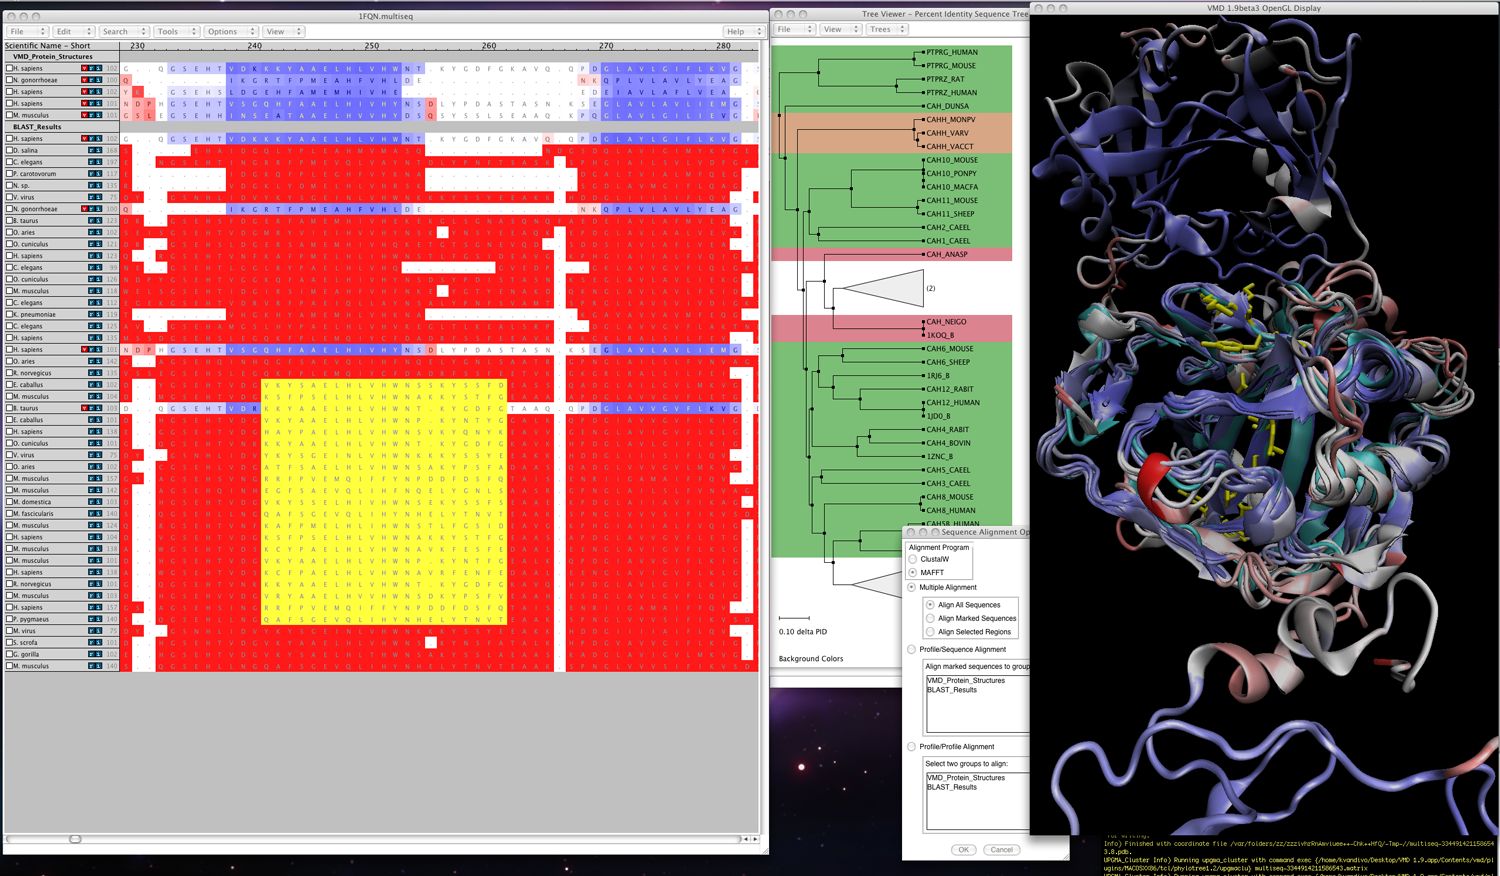
\includegraphics [width=5in]{./pictures/screenShot20110307.png}}
 \caption{MultiSeq In VMD}
\label{fullDisplay}
\end{figure}
article by O'Donoghue and Luthey-Schulten~\footnote {P.
O'Donoghue and Z. Luthey-Schulten. ``Evolution of Structure in
Aminoacyl-tRNA Synthetases''  MMBR, 67(4):550-73.  December, 2003. }
are part of MultiSeq.   In particular,  the Luthey-Schulten
group has included a structure-based measure of
homology \begin{math} Q_H \end{math} (see Appendix B), that takes into
account the effect of insertions and deletions and has been shown to
produce accurate structure-based phylogenetic trees.  The STAMP
structural alignment algorithm, kindly provided by our colleagues
Russell and Barton, is included~\footnote {R.B.
Russell and G.J. Barton. ``Multiple protein sequence alignment from
tertiary structure comparison: assignment of global and residue
confidence levels.''  Proteins: Struct. Func. Genet., 14:309-323.  1992.
}.  
%We plan to offer biomedical researchers a tool to examine the
%changes in protein structure in the correct statistical framework.  
As a result, Multiple Alignment is an invaluable tool for relating
protein structure to its function or misfunction.

In any publication of scientific results based completely or in part on
the use of MultiSeq, please reference:

Elijah Roberts, John Eargle, Dan Wright, and Zaida Luthey-Schulten.
MultiSeq: Unifying sequence and structure data for evolutionary
analysis.  BMC Bioinformatics, 2006, 7:382.


\subsection{Installation}
MultiSeq is part of the standard VMD release.  You can download VMD
from \texttt{http://www.ks.uiuc.edu/Research/VMD/}.  Although BLAST is
not necessary for the overall function of MultiSeq, it is highly
recommended to have BLAST installed locally (i.e. accessible through
file browsing on your local computer).  See
\texttt{http://www.scs.illinois.edu/\~{}schulten/multiseq/} for links to
tutorials with additional information on BLAST installation.

ClustalW is the default sequence alignment tool and is packaged with
MultiSeq.  However, MAFFT (available from
\texttt{http://mafft.cbrc.jp/alignment/software/}) can be used for doing
sequence alignment if it is installed on your computer system.  (MAFFT
version 6.811 has been tested.  Newer versions are expected to work as
well and should be used if possible.)

Paths to all locally installed software and databases are set via the
\textsf{File} | \textsf{Preferences} menu in the MultiSeq window.  The
\textsf{Preferences} menu has a `Metadata' tab and a `Software' tab.
The `Software' tab is where file paths can be provided.

MultiSeq uses a collection of databases that need to be downloaded to
your computer system.  The first time you run MultiSeq you
will be asked to create a folder to store these databases, and the
databases will then be downloaded from our servers.  When you
subsequently run the plugin, it will check to insure that you have the
most recent versions of the databases.



%\clearpage

% A review of the MultiSeq main window
% Go over the shortcuts and so forth
% We should create an in-depth image with indicators of what is what
\label{unit1}
% A review of the MultiSeq main window
% Go over the shortcuts and so forth
% We should create an in-depth image with indicators of what is what

\section{The MultiSeq Graphical Environment}
MultiSeq is accessed as an extension within VMD.  To begin MultiSeq,
launch VMD and:
\begin{enumerate}
\item In the VMD main window, click on the \textsf{Extensions} Menu.
\item In Extensions, select \textsf{Analysis} $\rightarrow$
\textsf{MultiSeq}.
\end{enumerate}
(alternatively, if you are a fan of command lines, you can type
`\texttt{multiseq}' into the VMD terminal window)

The main MultiSeq window (see Fig.~\ref{fig:main}) will appear (note
that the first time you run MultiSeq, you will be prompted to download
necessary databases before seeing the main window).

\begin{figure}[here]
 \centerline{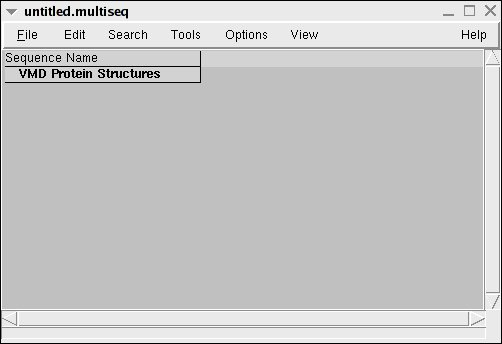
\includegraphics [width=5in]{./pictures/main_window.jpg}}
 \caption{Main MultiSeq Window With No Structures Loaded}%more information in caption about views etc.
\label{fig:main}
\end{figure}

%\subsection{MultiSeq Window Shortcuts}
%The main MultiSeq window has several shortcuts that provide complementary information with 
%additional functionality for the analysis of alignments.  For the purposes of examining these shortcuts, we will 
%use several structure and sequence files of the catalytic domain of AARSs.  
% The image with shortcut indicators will be around here


% Loading Data into MultiSeq
% bkd 8/2 - I believe this warrants having its own section since there are multiple ways of doing this. i.e., Import Data
% Detail doing a BLAST search 
\label{unit2}
% Loading Data into MultiSeq
% bkd 8/2 - I believe this warrants having its own section since there 
%are multiple ways of doing this. i.e., Import Data
% Detail doing a BLAST search

\section{Using and Managing Data}
To begin analyzing proteins in MultiSeq, data from
sequence\footnote{FASTA files.} and
structure\footnote{The ASTRAL database (http://astral.stanford.edu) is a
compendium of protein domain structures derived from the PDB database.
It divides each protein structure into its domain components. For
example, AspRS is divided into three separate PDB files: one containing
the catalytic domain, one with the insertion domain, and one for the
anticodon binding domain. The names of the files contain the PDB
extension, the letter a for ASTRAL, and a number, which corresponds to
which domain it is in the original PDB file.  
%FASTA format is writing a sequence into basic text, such that the sequence can be used to conduct searches via programs like BLAST.
%The Protein Data Bank (PDB) is an archive of experimentally determined three-dimensional structures of biological macromolecules, serving a global community of researchers, educators, and students. The archives contain atomic coordinates, bibliographic citations, primary and secondary structure information, as well as crystallographic structure factors and NMR experimental data.
The PDB is the single worldwide repository for the processing and
distribution of 3-D structure data of large molecules of proteins and
nucleic acids.} files is required.  Import Data (from the File menu
within MultiSeq) allows you to load
structure and sequence files, both locally and via a network connection.

Various structure and trajectory files, such as PDB and PSI, can be
loaded via the \textsf{New Molecule} function of the VMD Main window,
but \textsf{Import Data} allows you to load sequence files as well.
Additionally, Import Data has BLAST searching capabilities, if a local
copy of BLAST is installed.  

\begin{figure}[here]
 \centerline{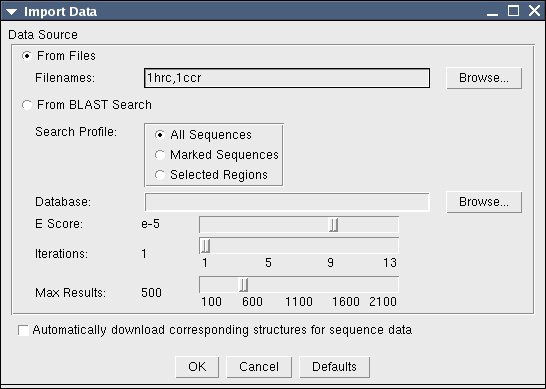
\includegraphics [width=5in]{./pictures/import_data.jpg}}
 \caption{Import Data Window}%more information in caption about views etc.
\label{importData}
\end{figure}
\subsection{Importing from files}
Structure\footnote{See VMD Manual for supported formats} and Sequence
files can be loaded into MultiSeq via \textsf{Import Data}.  PDB files are
structure files, whereas FASTA is a sequence file format.  To load these
files:
\begin{enumerate}
\item Make sure \textsf{From Files} is selected as a \textsf{Data
Source}.
\item In the \textsf{Filenames:} dialogue, either type in the location of the
file, or hit the browse button to locate the file.  Another option 
is to simply type in the PDB or SCOP id.  This option requires
a network connection for your computer to obtain files from PDB or
ASTRAL directly.
\item Hit the \textsf{OK} button.
\end{enumerate}
\noindent
If you would like to load multiple files/structures/sequences at once, 
you can separate each with a comma.\\

\subsection{Sequences and BLAST searching}
You can conduct a BLAST search from within MultiSeq if you have the
BLAST program installed on your computer.  You will need to install
BLAST if you haven't already done so, and you will have to configure
MultiSeq to know where BLAST is installed (via \textsf{File} |
\textsf{Preferences} | \textsf{Software})  

\begin{enumerate}
\item Before you open the \textsf{Import Data} window, you have the option of
either selecting a set of sequences, or a region within a sequence.
\item Go to \textsf{File} and then \textsf{Import Data} and select
\textsf{From BLAST Search}, 
and either \textsf{All Sequences}, \textsf{Marked Sequences}, or
\textsf{Selected Regions}.
\item In the \textsf{Databases}, either type the location of the
database, or use the \textsf{Browse} button to locate it.  This could be
something like a Swiss PROT database or otherwise.  Once you give
MultiSeq the name of a database, it will remember it for future
searches.  
\item Select the \textsf{E Score}, \textsf{Iterations}, and \textsf{Max
Results}.
\item If you want MultiSeq to automatically download structure
information for sequences found via the BLAST search, mark the checkbox
for that.
\item Hit the \textsf{OK} button.
\end{enumerate}

\begin{figure}[here]
\centerline{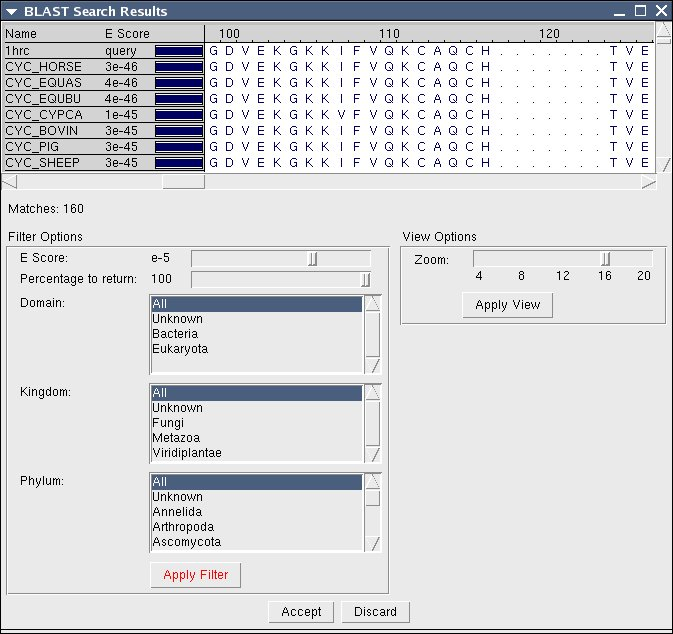
\includegraphics [width=5in]{./pictures/BLAST_results.jpg}}
 \caption{BLAST Search Results}%more information in caption about views etc.
\label{blast}
\end{figure}

MultiSeq will then begin a BLAST search.  This may take several minutes.
When the search is done, a new window called \textsf{BLAST Search
Results} will appear.  The results do not immediately appear in the main
MultiSeq window, because you can apply further filters on the retrieved
sequences.  The \textsf{BLAST Search Results} window is divided into
three main parts: the sequence viewer, \textsf{Filter Options}, and
\textsf{View Options}.     

The sequence viewer is a read-only display of the sequences that match
your BLAST search.  The number of matches is listed below the sequence
viewer.

You can use the \textsf{Zoom} to change how much of each sequence you
see.  You can change the zoom level and \textsf{Apply View} and you will
see fewer or more sequences in the sequence viewer portion of the
window.

In the \textsf{Filter Options} you can tweak the parameters to reduce or
expand the number of sequence matches.  Once you have changed a
parameter you can hit \textsf{Apply Filter} and see which sequences
match.

Once you have a collection of sequences that you want to import, you can
hit the \textsf{Accept} button at the bottom and they will be added to
the MultiSeq window.




% Performing Alignments?
% detail doing both types of alignments
% maybe a para on organizing sequences into groups within sequence display?
\label{unit3}
%Working in the MultiSeq Environment
\section{Working in the Environment}
MultiSeq provides a unique working environment for the analysis of
proteins.  

\subsection{Title Display}
By default, for each sequence loaded into Multiseq, you will be shown
the ``sequence name'' as the title for each row in the main window.
Sometimes this is not as useful as, for instance, the scientific name of
the sequence might be.  Multiseq allows you to change the displayed
title for each sequence by by left clicking on the header of the titles
and choosing a different option.  This can be seen in 
Figure~\ref{fig:title_display}.  
\begin{figure}[here]
 \centerline{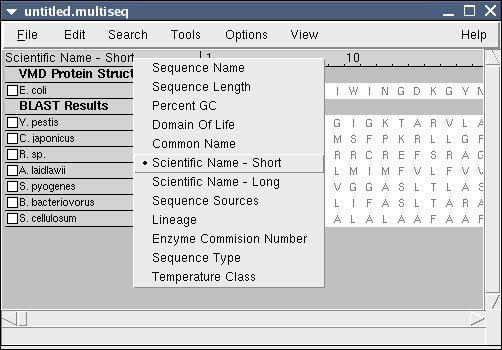
\includegraphics [width=3in]{./pictures/title_display.jpg}}
 \caption{Choosing Data To Display As Sequence Title}%more information in caption about views etc.
 \label{fig:title_display}
\end{figure}
If you choose an option where a sequence does not have a value, Multiseq
will show you the $<$Sequence Name$>$ in angle brackets.

\subsection{Grouping}
While working with the Sequence Viewer in MultiSeq, you may notice
certain patterns or trends.  As a result you would like to put certain
sequences closer to others to analyze such motifs.  MultiSeq allows such
grouping based on taxonomy or you can customize the groupings.  Right
clicking on a group name (such as \textsf{VMD Protein Structures} will bring
up a context menu where you can manage groups.

% \subsection{Managing Representations}

\subsection{Info Viewer}
Whenever you load a sequence or structure into MultiSeq an `\texttt{i}' box will
appear next to the protein's ID.  If you click on this box, a new
window will appear called the \textsf{Info Viewer} (See
Fig.~\ref{fig:editSeqInfoWindow}).  Within this window
information regarding the species the protein is from will appear. If
you have PSIPred installed and configured, you can predict the secondary
structure at the bottom of the Info window.
\begin{figure}[here]
 \centerline{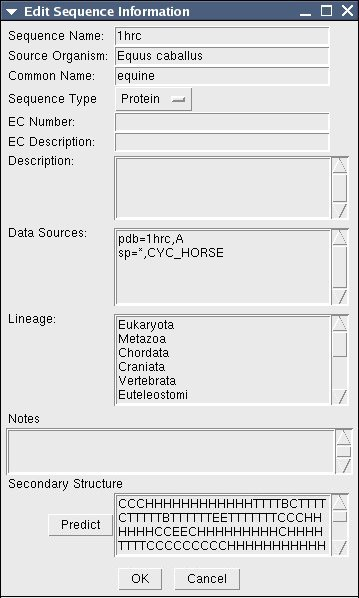
\includegraphics [width=3in]{./pictures/editSeqInfo.jpg}}
 \caption{Edit Sequence Information}%more information in caption about views etc.
 \label{fig:editSeqInfoWindow}
\end{figure}

\subsection{Selecting vs. Marking}
As you browse the menus of MultiSeq you will notice options for
\textsf{Selected Sequences} or \textsf{Marked Sequences}.  ``Selecting
Sequences'' is when you highlight a portion of the sequence(s) in the
sequence viewer using the mouse.  This can be either the entire sequence
or a portion.  However ``Marking Sequences'' allows you to more easily
select an entire sequence by simply checking the box next to the protein
ID.







\section{Edit Menu}

Along with the copy/cut/paste options that you expect to see in an edit
menu, this menu also provides a power sequence editor.

If you want to edit a sequence, \textsf{Enable Editing}.  If you are
just wanting to align sequences, you can probably choose to just enable
gap editing.  Once you have enabled editing, you can then use the mouse
to choose a residue (or residues).  Hit the space bar to insert a gap,
or, if you have enabled full editing, you can insert a residue by typing
the desired character.

If you want to truly edit the sequences manually, you can choose to
\textsf{Edit In Text Editor}.  VMD's text editor will be loaded, and you
can change the sequence data.  Dashes are gaps and the sequence
characters can be changed as you see fit.




\label{unit8}

% Search Menu

\section{Search Menu}

\begin{description}
\item [Find, Find Next, Find Previous] Via \textsf{Search}, you can find
and highlight residues in sequences. When you use \textsf{Find}, all of
the residues will be highlighted, and you can then cycle through them by
using \textsf{Find Next} and \textsf{Find Previous}.

\item[Select Contact Shells]
See Figure~\ref{fig:select_cs}.
 \begin{figure}[here]
 \centerline{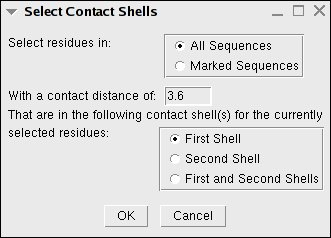
\includegraphics [width=3in]{./pictures/select_contactshells.jpg}}
 \caption{Select Contact Shell Window}
\label{fig:select_cs}
\end{figure}

\begin{description}
     \item[Select residues in:] Lets you choose whether to look through
     all sequences, or just the ones you have marked.
     \item[With a contact distance of:] defaults to 3.6.
     \item[That are in the following contact shell(s) for the currently
     selected residues] Choose from \textsf{First}, \textsf{Second}, or
     \textsf{First and Second} shells
\end{description}     

\item[Select Non-Redundant Set]

You can use structure QR or sequence QR to select a non-redundant set
(See Fig.~\ref{fig:select_nr}).

 \begin{figure}[here]
 \centerline{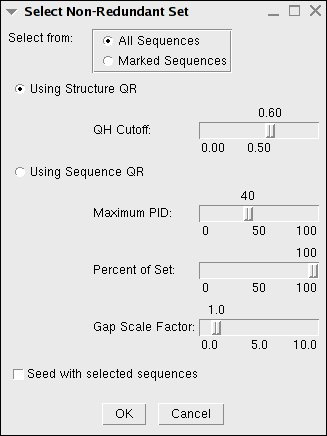
\includegraphics [width=3in]{./pictures/select_nrset.jpg}}
 \caption{Select Non-Redundant Set Window}
\label{fig:select_nr}
\end{figure}

% foobar.  Needs detail
\begin{description}
     \item[Select from:] Lets you choose whether to look through
     all sequences, or just the ones you have marked.
     \item[Using Structure QR]
          \begin{description}
               \item[QH Cutoff:]  Can vary from 0 to 1.
           \end{description}
    \item[Using Sequence QR]
             \begin{description}
               \item[Identity Cutoff:]
               \item[Gap Scale Factor:]
           \end{description}   
     \item[Seed with selected sequences]  If you have selected certain
     sequences, you can seed the algorithm with these sequences to
     select a non-redundant set based on them.
\end{description}

\item[Select Residues]
The \textsf{Residue Selection} feature (See
Fig.~\ref{fig:select_res})lets you analyze conservation, using different
measures, and highlight residues in the Sequence Display and Structure
Display simultaneously.  \textsf{Residue Selection} allows you to examine the
conservation on a per residue basis.
 
\begin{figure}[here]
\centerline{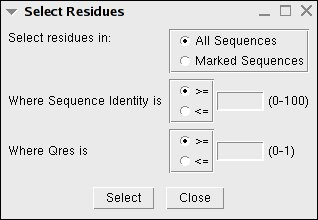
\includegraphics[width=3in]{./pictures/select_residues.jpg}}
\caption{Select Residues Window}%more information in caption about views
etc.  \label{fig:select_res} \end{figure}

There are two options: either \textsf{Where
Sequence Identity is} or \textsf{Where Qres is}.  \textsf{Where Sequence
Identity is} is a sequence identity measure, whereas \textsf{Where Qres
is} is a structure measure.

\begin{description}
     \item[Select residues in:] You can choose all sequences or just the
     marked ones.
     \item[Where Sequence Identity is:] If this option is selected you
     can select `less than or equal to' or `greater than or equal to' 
     option, then a number
     between 0-99.
     \item[Where Qres is:] If this option is selected you 
     can select `less than or equal to' or `greater than or equal to' 
     option, then a number between zero and one.
\end{description}
\end{description}



\section{Tools Menu}

\subsection {Performing Alignments}
MultiSeq can do both structural and sequence alignments.  These options
are available via the \textsf{Tools} menu in MultiSeq.

% Performing Alignments?
% detail doing both types of alignments
% maybe a para on organizing sequences into groups within sequence 
%display?

%I believe I have the majority of this subsection down, but John really ought to go over this 
\subsubsection {Structure Alignments}
MultiSeq uses the program STAMP to structurally align protein molecules.
The STAMP algorithm minimizes the $C_\alpha$ distance between aligned
residues of each molecule by applying globally optimal rigid-body
rotations and translations. Also, note that you can perform alignments
on molecules that are structurally similar. If you try to align proteins
that have no common structures, STAMP will have no means to align them.
If you would like further information about how the alignment occurs,
please refer to the STAMP manual.
\begin{figure}[here]
 \centerline{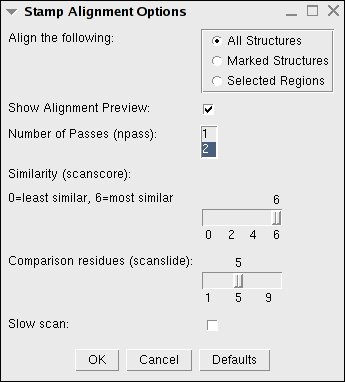
\includegraphics [width=3in]{./pictures/stamp.jpg}}
 \caption{STAMP Structural Alignment Window}%more information in caption about views etc.
 \label{stampWindow}
\end{figure}
\begin{description}     
      \item [Align the following:] Choose which structures you wish to
      align
      \item [Number of passes (npass):] Whether one or two fits are to
      be performed. The idea is that the initial fit can be used with a
      conformation biased set of parameters to improve the initial fit
      prior to fitting using distance and conformation parameters.
      Default NPASS = 1
      \item [Similarity (scanscore):] Specifies how the Sc value (STAMP
      algorithm) is to be calculated. This depends on the particular
      application. As a general rule of thumb, use SCANSCORE=6 for large
      database scans, when you are scanning with a small domain, and
      wishing to find all examples of this domain - even within large
      structures. Use SCANSCORE=1 when you wish to obtain a set of
      transformations for a set of domains which you know are similar
      (and have defined fairly precisely as domains rather than the
      larger structure that they may be a part of). Default SCANSCORE =
      6
      \item [Comparison residues (scanslide):] This is the number of
      residues that a query sequence is 'slid' along a database sequence
      to derive each initial superimposition. Initially, the N-terminus
      of the query is aligned to the 1st residue of the databse, once
      this fit has been performed and refined, and tested for good
      structural similarity, the N-terminus is aligned with the 1+th
      position, and the process repeated until the end of the database
      sequence has been reached. Default SCANSLIDE = 5
      \item [Slow scan:] If set to TRUE, then the SLOW method of getting
      the initial fits for scanning will be used (See chapter 1).
      Default SLOWSCAN = FALSE
      \item [Defaults:] resets the STAMP parameters to their original values
\end{description}


%Elijah, I'll need assistance with the description of Sequence Alignments and soon will be adding
%directions for running an alignment

\subsubsection {Sequence Alignments}

Sequence alignment in MultiSeq can be done via ClustalW or MAFFT (if you
have MAFFT locally installed) (See Fig.~\ref{seqAlignMenuWindow}).

 \begin{figure}
 \centerline{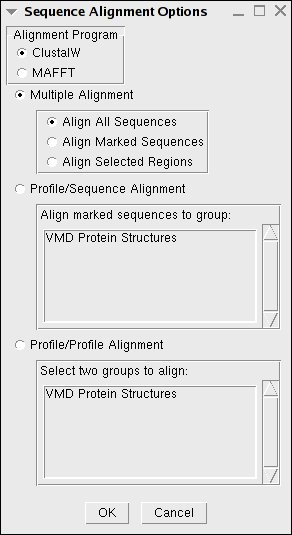
\includegraphics {./pictures/sequenceAlignmentMenu.jpg}}
 \caption{Sequence Alignment Menu Window}
\label{seqAlignMenuWindow}
\end{figure}

Once you have decided which program to use (you won't be able to select
MAFFT if you haven't configured the path to MAFFT on your local computer
via \textsf{File} | \textsf{Preferences} | \textsf{Software}), you can 
choose from 
Multiple Alignment, Profile/Sequence Alignment, or
Profile/Profile Alignment.  Once you have chosen the desired type
of alignment, you can set the proper option.

\begin{description}
     \item[Multiple Alignment]  Choose which sequences or regions you
     wish to align.
     \item[Profile/Sequence Alignment] This requires certain sequences
     to be marked, and they will then be aligned to the group that you
     specify.
     \item[Profile/Profile Alignment] To align one entire group with
     another entire group, select this option.
\end{description}

If you choose MAFFT, be aware of the following:
\begin{itemize}
\item MultiSeq has been tested with MAFFT version 6.811.  It should work
with any version of MAFFT reasonably close to that.
\item MultiSeq uses the default \textsf{-auto} option for MAFFT.
\item Profile-profile and sequence-profile alignment will be done with
MAFFT if it is chose as the desired alignment program.
\item When configuring the path to MAFFT, you need to give the path to
the `bin' directory on a unix-type system.  On Windows, give the path
that contains the `mafft.bat' file.
\end{itemize}




% Tools Menu

%need result/dendogram windows 

\subsection{Phylogenetic Tree}
The Phylogenetic Tree feature helps in determining the
structure and sequence-based relationships between the aligned domains
of proteins.\\ ~\\ To do this, it uses a modification of Q that accounts
for both gapped and aligned regions.  This new metric, \begin{math} Q_H
\end{math}, creates a structure-based phylogeny that is congruent to the
\begin{figure}[here]
 \centerline{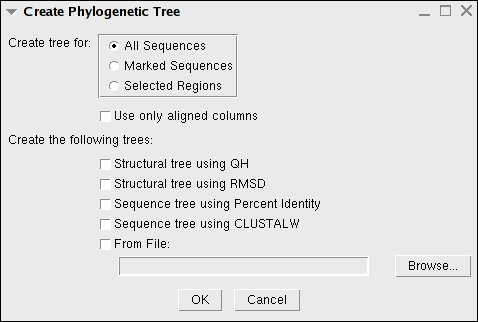
\includegraphics [width=3in]{./pictures/ptree1.jpg}}
 \caption{Create Phylogenetic Tree Window}
\label{fig:ptree1}
\end{figure}
sequence-based phylogenies.  You can create a Phylogenetic Tree from the
\textsf{Tools} menu in MultiSeq (See Fig.~\ref{fig:ptree1}).  Once you
choose the sequences or regions you wish to create a tree for, you can
choose which trees you want to create.  The tree viewer can also create
a tree from a data file that you provide (if you have created tree data
from an external program, for instance).

Once you have chosen which trees to create, the Tree Viewer will be
shown in simple black and white.  But, you can easily use color and Tree
View commands to make the data more useful (see Fig.~\ref{fig:ptreeView}).  
\begin{figure}[here]
 \centerline{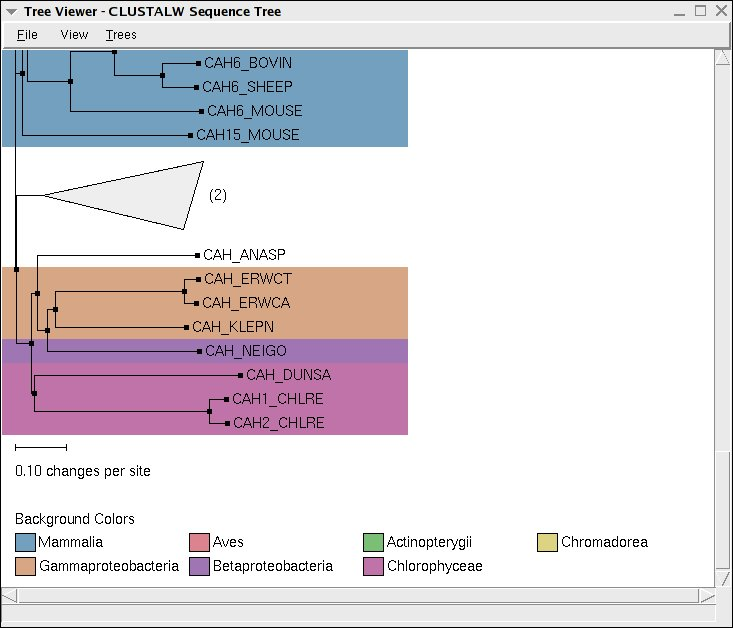
\includegraphics [width=3in]{./pictures/ptreeView.jpg}}
 \caption{Phylogenetic Tree Viewer - CLUSTALW Sequence Tree}
\label{fig:ptreeView}
\end{figure}

The Tree Viewer window is very powerful.  In the main window, you can
right click on any small black box (in front of an individual sequence,
or at any joint in the tree) and remove the element/subtree or look at
its properties.  Additionally, if you have selected a subtree, you can
change the shape of the tree.  You can collapse/expand a subtree, as
shown in Fig.~\ref{fig:ptreeView} as well.

Menu options include:

\begin{description}
\item[File]  Trees can be loaded and saved in common formats.
Additionally, postscript renderings can be created for use in
publications.
\item[View] If a distance matrix has been created from the data, you can
view it.  You can also modify the way the tree looks.  You can zoom in
and out, change the scale (which pushes tree leaves left or right for
viewability).  Orientation will move the labels from the left side of
the tree to the right, and you can even choose whether or not you wish
the tree to display the labels and nodes.

The \textsf{Leaf Text} option lets you choose the labels that you wish
to have displayed, and you can color the labels as well as the tree
backgrounds by a variety of different metrics. 

You can easily collapse large parts of the tree by choosing a criteria,
and, if you have selected a point in the tree, you can make that point
the new root node of the tree.

\item[Trees] If you have chosen to create multiple trees, you can use
this menu to rotate through the trees, or you can jump to one directly.

\end{description}
%\subsubsection{Print QR ordering}
%\subsection{Plot Data}
%\subsubsection{RMSD Tools}
%\subsubsubsection{RMSD per Residue}
%The ability to graphically display the RMSD per Residue between two proteins is a useful feature for demonstrating how well the proteins align.
%The root mean square deviation (RMSD) measures the distances in angstroms between the C-alpha atoms of 2 aligned residues.\\
%\subsubsubsection{Pairwise RMSD}
%Pairwise RMSD prints the average overall RMSD for each pair of aligned proteins.


% Tools Menu

%need result/dendogram windows 

\subsection{Plot Data}
\textsf{Plot Data} 
create graphs of internal MultiSeq data.
\begin{figure}[here]
 \centerline{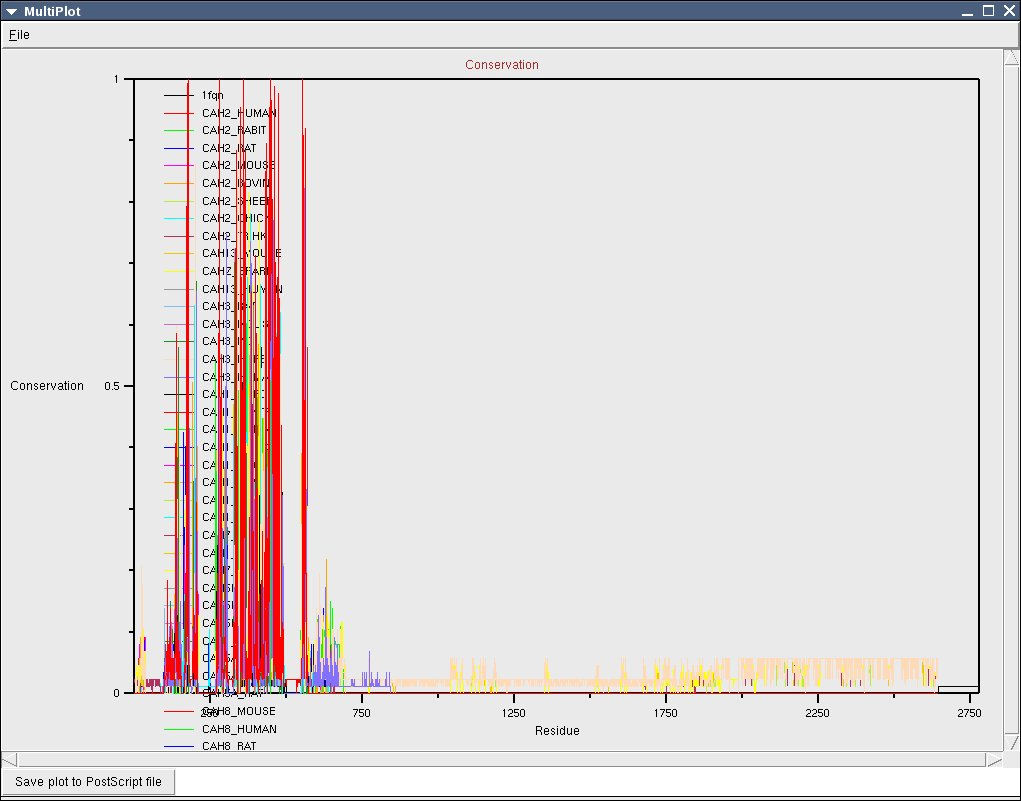
\includegraphics [width=3in]{./pictures/multiPlot.jpg}}
 \caption{Plot Data - Sequence Conservation}
\label{fig:plotData}
\end{figure}
You can \textsf{Plot Data} from the \textsf{Tools} menu in MultiSeq.
Once you choose the sequences or regions you wish to plot, you can
choose the data (such as \textsf{Qres}, \textsf{RMSD}, etc) for each
residue that you want to display.  You can also plot custom data.  The
data graph will then be displayed (see Fig.~\ref{fig:plotData}).  If you
wish, you can create a postscript file for publication.







\label{unit7}

\section{Options Menu}

\begin{description}
% foobar.  Need atom picking text
\item[Atom Picking] Normally disabled, but can be turned on.
\item[Grouping] MultiSeq can automatically create groups and show the
sequences in the MultiSeq window sorted accordingly.  Just choose the
grouping that you want to use.
\end{description}



% View Menu
\label {unit4}

% View Menu

\section{View Menu}

The \textsf{View} menu provides several useful options for coding and
looking at large amounts of data.

\begin{itemize}
\item[Zoom] To change the amount of data seen in the MultiSeq window,
you can zoom in and out.  As you zoom farther out (choosing a percentage
that is smaller) MultiSeq will makes the sequence letters smaller and
smaller until you will only see the background colors and then, not even
that.  If you need to see the entire sequence, the \textsf{Zoom Window},
discussed below, might be more useful.
\item [Coloring]
You can choose to color the sequences by a wide range of attributes.
First, you can choose \emph{what} you want to color by choosing
\textsf{Apply to All}, \textsf{Group}, or \textsf{Marked}.  Then, you
can choose the coloring method that you wish to apply.  

For \textsf{Qres}, traditionally, Q has meant ``the fraction of
     similar native contacts'' between the aligned residues in two
     proteins\footnote {Eastwood, M.P., C. Hardin, Z. Luthey-Schulten,
     and P.G. Wolynes. ``Evaluating protein structure-prediction schemes
     using energy landscape theory.''  IBM J . Res. Dev. 45: 475-497.
     2001}, or in two different conformational states of the same
     protein.  When Q = 1, it indicates that the structures are
     identical.  When Q has a low score (\textit{0.1}), it means the
     structures do not align well, or, in other words, only a small
     fraction of the C-alpha atoms superimpose.  You will discover that
     homologs typically have Q$\ge$0.4.  Q per residue is the
     contribution from each residue to the overall average Q score.  For
     more information see Appendix A.

For \textsf{Sequence Identity}, the aligned domains are colored by how
much of the sequence is conserved. The \textsf{Sequence Identity}
coloring method colors each amino acid according to the degree of
conservation within the alignment: blue means highly conserved, wheras
red means very low or no conservation.

\item[Highlight Style]
\textsf{Highlight Style} is an option for the OpenGL diplay.  The style
refers to drawing method in VMD\footnote {For more information about
drawing methods, please refer to the VMD manual.}.  This option allows a
user to highlight residues of a structure in the sequence display and
see the areas simultaneously highlighted in the OpenGL display.

\item[Highlight Color]
\textsf{Highlight Color} is another option for the OpenGL diplay.
Alongside \textsf{Highlight Style}, \textsf{Highlight Color} is the
color or coloring method\footnote{For more information, please refer to
the VMD manual} used in the OpenGL display when highlighting residues in
the Sequence Display.  The default \textsf{Highlight Color} is yellow.

\item[Color Scale]  Once you have chosen a coloring, you might wonder
what the specific colors mean.  The \textsf{Color Scale} option will
show you the scale of colors according to value.

\begin{figure}[here]
 \centerline{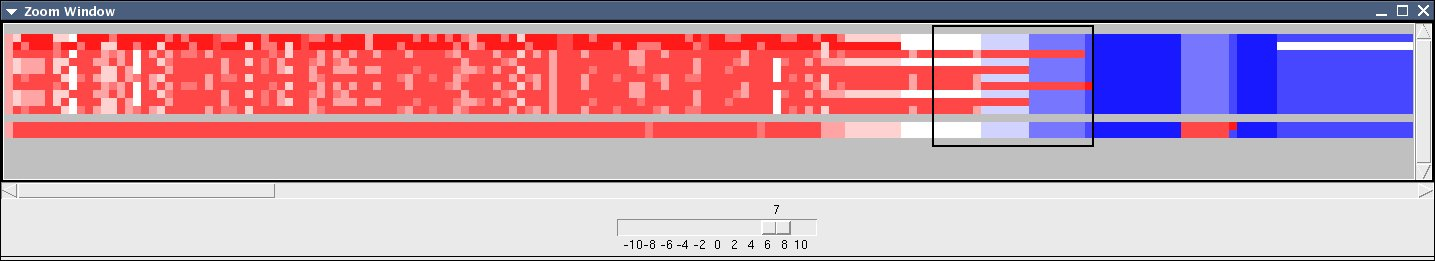
\includegraphics [width=5in]{./pictures/zoomWindow.jpg}}
 \caption{Zoom Window}
\label{fig:zoomWindow}
\end{figure}
\item [Zoom Window] (See Fig.~\ref{fig:zoomWindow}) If you need to see
the entire collection of sequences and quickly move from area to area,
the \textsf{Zoom Window} will be useful to you.  It shows the entire
sequence palette.  You can choose the zoom factor using the sliding bar
at the bottom of the window, and the black box shows you the area of the
sequences that are currently visible in the MultiSeq window.  To see
other areas, just click the mouse and the black box will be moved to the
mouse pointer location.

Note:  When you have the \textsf{Zoom Window} open, the MultiSeq window
will redraw more slowly.  If this is a problem for you, just close the
\textsf{Zoom Window} and reopen as needed.

\end{itemize}



\label{unit9}

% Saving Data from MultiSeq sessions
%We just need to figure out what we're doing with this
\section{Working With Sessions}
The \textsf{Load} and \textsf{Save Session} options from the
\textsf{File} menu provide a way to save and load all of the files,
alignments, and visual representations currently in use within MultiSeq
in a convenient package.  

\subsection{Save Session}
You can save a session of MultiSeq, with all of the files, alignments,
and visual representations, by simply going to the \textsf{File Menu}
and selecting \textsf{Save Session}.  You will be prompted to save the
session, and will have the opportunity to create a unique name for the
session here.  Hit the \textsf{OK} button.  A file will be generated
with a \texttt{.multiseq} extention along with a directory filled with
various files necessary to load the saved session into MultiSeq.  Please
note that both the generated file and directory have to be in the same
directory location in order to load up the session in the future
properly.  

\subsection{Load Session}
Unlike \textsf{Import Data} (also in the \textsf{File} menu),
\textsf{Load Session} opens up a previous session of MultiSeq with all
of the sequence and structure files aligned, and using previous coloring
and drawing methods.  To load a previously saved MultiSeq Session,
simply select the \textsf{File} menu and \textsf{Load Session}.  A file
broswer will appear allowing you to select a file with the extension
\texttt{.multiseq} and make sure it has a corresponding directory of the
same name.

\section{Other Ways To Export Data}

\subsection{Save to PostScript}  From the \textsf{File} menu, if you
choose \textsf{Save Screenshot}, you will be able to save a postscript
version of the MultiSeq window.
%\subsection{Write PDB from selection...}
%During a MultiSeq session, you  may want to save various persepectives
%of the structural alignments you created.  Often these images are
%generated by highlighting specific portions of the aligned protein
%sequences. If you would like to study your selections further, you can
%can do so by generating your own PDB file(s).  To begin this process:
%\begin{enumerate}
%\item Highlight the portions of the sequence that you want to examine in
%the Sequence Display of the MultiSeq window.
%\item In the same window top pull-down menu, go to View$\rightarrow$
%Highlight style. Multiple Highlight styles will appear to choose from.
%Select one and make sure it appears in the OpenGL Display.
%\item Click on File $\rightarrow$Write PDB from selection....
%\item The PDB file(s) will be saved in a directory that can be chosen by
%clicking on the File $\rightarrow$ Choose Work Directory.... If you
%have not selected your Work directory, you be prompted to choose a
%directory when you click on Write PDB from selection....
%\end{enumerate}
%\subsection{Save work data into another directory...}


 

\label{unit10}

%should add information on QR

\section{Appendices}
\subsection{Appendix A: $Q$}
The following equation is from the article ``Evaluationg protein
structure-prediction schemes using energy landscape theory'' by
Eastwood, et al.

\[
Q=\frac{2}{\ (N-1)(N-2)} \sum _{i<j-1}\exp \left[ -\frac{\left( r_{ij}-r^{N}_{ij}
\right)^{2}}{2\sigma ^{2}_{ij}}\right] 
\]

\noindent
$r_{ij}$ is the distance between a pair of $C^{\alpha}$ atoms.\\
~\\
$r_{ij}^N$ is the $C^{\alpha}$-$C^{\alpha}$ distance between residues 
$i$ 
and $j$ in the native state.\\
~\\
$\sigma ^{2}_{ij}=\left| i-j\right| ^{0.15}$ is the standard deviation, determining the width of the Gaussian function.\\
~\\
$N$ is the number of residues of the protein being considered.


\newpage
\subsection{Appendix B: $Q_H$}
The following text is in the article ``On the evolution of structure in 
aminoacyl-tRNA synthetases.''
by O'Donoghue et al.\\

\begin{center}
{\bfseries Homology Measure}
\end{center}
~\\
We employ a structural homology measure which is based on the structural
similarity measure, {\it Q}, developed by Wolynes, Luthey-Schulten, and
coworkers  in the field of protein folding. Our adaptation of {\it Q} is
referred to as $Q_H$, and the measure is designed to include the effects
of the gaps on the aligned portion: $Q_H$=$\aleph$($q_{aln}$+$q_{gap}$),
where $\aleph$ is the normalization, specifically given below.  $Q_H$ is
composed of two components. $q_{aln}$ is identical in form to the
unnormalized {\it Q} measure of Eastwood et al. and accounts for the
structurally aligned regions. The $q_{gap}$ term accounts for the
structural deviations induced by insertions in each protein in an
aligned pair: 
 
%\begin{center} \begin{figure}[here]
%\centerline{\includegraphics{./pictures/qh.pdf}} \end{figure}
%\end{center} \noindent
\[Q_{H}=\aleph \left[ q_{aln}+q_{gap}\right] \]

\[
q_{aln}=\sum _{i<j-2}\exp \left[ -\frac{\left( r_{ij}-r_{i^{\prime }j^{\prime }}
\right)^{2}}{2\sigma ^{2}_{ij}}\right] 
\]


\begin{eqnarray}
q_{gap} &=& \sum _{g_{a}}\sum ^{N_{aln}}_{j}\max \left\{ \exp 
\left[ -\frac{\left( r_{g_{a}j}-r_{g^{\prime}_{a}j^{\prime}}\right)^{2}}
{2\sigma ^{2}_{g_{a}j}}\right] ,\exp \left[ -\frac{\left( r_{g_{a}j}-r_{g^{\prime \prime }_{a}j^
{\prime }}\right) ^{2}}{2\sigma ^{2}_{g_{a}j}}\right]\right\}\nonumber\\
&+& \sum _{g_{b}}\sum ^{N_{aln}}_{j}\max \left\{ \exp \left[ -\frac
{\left( r_{g_{b}j}-r_{g^{\prime}_{b}j^{\prime}}\right)^{2}}{2\sigma ^{2}_{g_{b}j}}\right] ,
\exp \left[ -\frac{\left( r_{g_{b}j}-r_{g^{\prime \prime }_{b}j^{\prime }}\right) ^{2}}
{2\sigma^{2}_{g_{b}j}}\right] \right\} \nonumber
\end{eqnarray}

The first term, $q_{aln}$, computes the unnormalized fraction of
$C^{\alpha}$-$C^{\alpha}$ pair distances that are the same or similar
between two aligned structures. $r_{ij}$ is the spatial
$C^{\alpha}$-$C^{\alpha}$ distance between residues $i$ and $j$ in
protein a, and $r_{i'j'}$ is the $C^{\alpha}$-$C^{\alpha}$ distance
between residues $i$' and $j$' in protein b. This term is restricted to
aligned positions, e.g., where $i$ is aligned to $i$' and $j$ is aligned
to $j$'.  The remaining terms account for the residues in gaps. $g_a$
and $g_b$ are the residues in insertions in both proteins, respectively.
${g'}_{a}$ and ${g''}_{a}$ are the aligned residues on either side of
the insertion in protein a. The definition is analogous for ${g'}_{b}$
and ${g''}_b$.\\ The normalization and the \(\sigma ^{2}_{ij} \) terms
are computed as:

\[
\aleph =\frac{1}{\frac{1}{2}\left( N_{aln}-1\right) \left( N_{aln}-2\right) +N_{aln}N_{gr}-n_{gaps}-2n_{cgaps}}\]


\[
\sigma ^{2}_{ij}=\left| i-j\right| ^{0.15} 
\]


where~\( N_{aln} \) is the number of aligned residues. \( N_{gr} \) is
the number of residues appearing in gaps, and \( n_{gaps} \) is sum of
the number of insertions in protein ``a'', the number of insertions in
protein ``b'' and the number of simultaneous insertions (referred to as
bulges or c-gaps). \( n_{cgaps} \) is the number of c-gaps. Gap-to-gap
contacts and intra-gap contacts do not enter into the computation, and
terminal gaps are also ignored. \( \sigma ^{2}_{ij} \) is a slowly
growing function of sequence separation of residues \( i \) and \( j \),
and this serves to stretch the spatial tolerance of similar contacts at
larger sequence separations. \(Q_{H}\) ranges from 0 to 1 where
\(Q_{H}=1\) refers to identical proteins. If there are no gaps in the
alignment, then \( Q_{H} \) becomes \( Q_{aln}=\aleph q_{aln}\), which
is identical to the Q-measure described into the $Q$ measure described
before.



\end{document}





